\section{Controller design with disturbance on the output}
\label{system_design_implementation}


As mentioned in \secref{control_intro}, a better control approach is to represent the state space model in discrete time in order to make it possible to implement on the system. In \figref{fig:block_dist}, an overview of the control design can be seen where the disturbance is on the output of the system and therefore not included in the state-space design.

\begin{figure}[H]
\centering
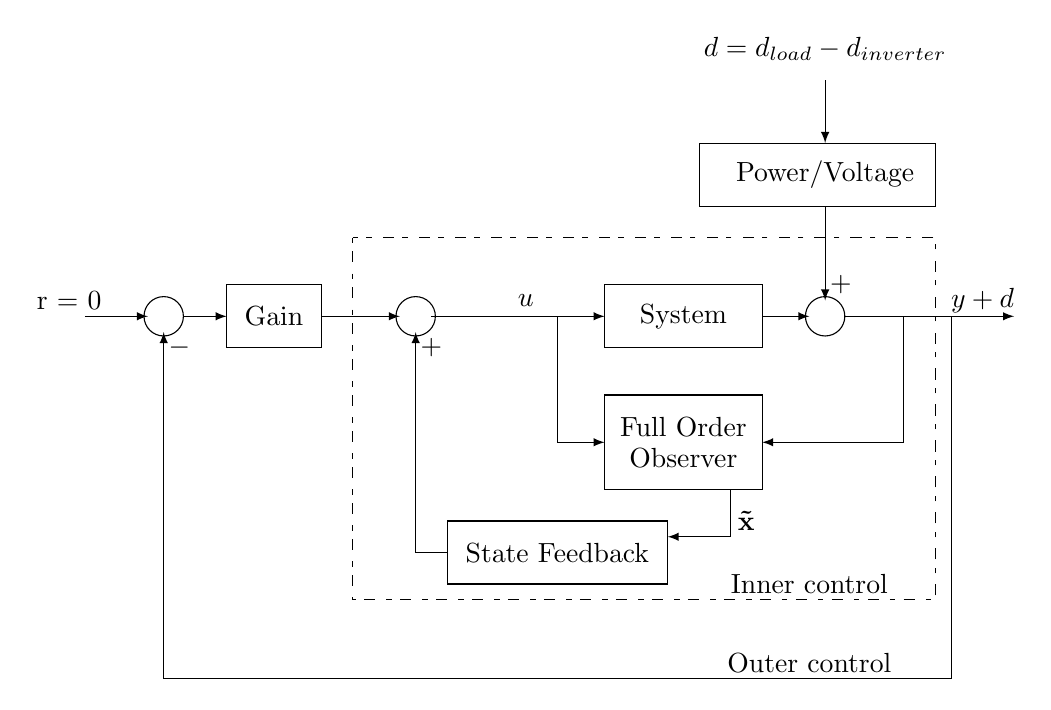
\begin{tikzpicture}
 \draw [-latex] (-1.4,2) ellipse (0.25 and 0.25);
 \node at (2,2) {\normalsize{System}};
\draw [-latex] (1,2.4) rectangle (3,1.6);
 \node at (2,0.2) {\normalsize{Observer}};
  \node at (2,0.6) {\normalsize{Full Order}};


\draw [-latex] (1,1) rectangle (3,-0.2);
\draw [-latex](-1.2,2) -- (1,2);
\draw [-latex](0.4,2) -- (0.4,0.4) -- (1,0.4);

\draw [-latex](4.8,2) -- (4.8,0.4) -- (3,0.4);

 \node at (0.4,-1) {\normalsize{State Feedback}};
 
 
\draw [-latex] (-1,-0.6) rectangle (1.8,-1.4);
\draw [-latex](2.6,-0.2) -- (2.6,-0.8) -- (1.8,-0.8);

\draw [-latex](-1,-1) -- (-1.4,-1) -- (-1.4,1.8);

  \node at (-3.2,2) {\normalsize{Gain}};


\draw [-latex](-2.6,2) -- (-1.6,2);
\node at (5.8,2.2) {\normalsize{$y+d$}};
\node at (0,2.2) {\normalsize{$u$}};

\node at (2.8,-0.6) {\normalsize{$\mathbf{\tilde{x}}$}};

\draw [-latex] (-3.8,2.4) rectangle (-2.6,1.6);

\draw [-latex] (-4.6,2) ellipse (0.25 and 0.25);

 \draw [-latex] (3.8,2) ellipse (0.25 and 0.25);

\draw [-latex](3,2) -- (3.6,2);
\draw [-latex](4.05,2) -- (6.2,2);
\draw [-latex](3.8,3.4) -- (3.8,2.2);



\draw [-latex](-4.35,2) -- (-3.8,2);
\draw [-latex](-5.6,2) -- (-4.8,2);
\draw [-latex](5.4,2) -- (5.4,-2.6) -- (-4.6,-2.6) -- (-4.6,1.8);

 \node at (3.8,5.4) {\normalsize{$d =d_{load}-d_{inverter}$}};
 
 \node at (4,2.4) {$+$};
\node at (-4.4,1.6) {$-$};
\node at (-5.8,2.2) {r = 0};

\draw [dash pattern=on 2pt off 3pt on 4pt off 4pt] (-2.2,3) rectangle (5.2,-1.6);
\node at (3.6,-1.4) {\normalsize{Inner control}};
\node at (3.6,-2.4) {\normalsize{Outer control}};

\draw [-latex] (2.2,4.2) rectangle (5.2,3.4);
\node at (3.8,3.8) {\normalsize{Power/Voltage}};
\draw [-latex](3.8,5) -- (3.8,4.2);
\node at (-1.2,1.6) {$+$};
\end{tikzpicture}


\caption{Block diagram of the system with disturbance.}
\label{fig:block_dist}
\end{figure}

The control has to deal with two control levels. The inner and outer control loops have to work together and reduce the effect of the disturbances. The state feedback sets the dynamics of the system. Therefore the feedback gain should be carefully chosen in order to avoid overreaction due to the disturbance in the outer loop. 

During the implementation, the voltage on the output is measured and the input signal for the system is known. For that reason, a full state observer is applied to calculate the states for the state feedback. 

The gain in the outer system serves as a scaling factor for the discrete system and helps improving the voltage error on the output. The reference of the system is set to zero because the error on the output should converge to zero without significant overshoots and as fast as it is possible. 
